% Electronica agropecuaria
%Tal y como se menciona en el capitulo 2, el objetivo principal de este proyecto radica en el desarrollo de un sistema tal que ayude, permita y facilite el monitoreo alimenticio de un conjunto de novillos estabulados en proceso de engorde; para ello primero es necesario comprender las etapas que influyen en la adquisición de datos y posteriormente considerar oportunidades de intervención (OI) o mejora desde un punto de vista ingenieril.\\

A modo general, en el capítulo anterior se habló del contexto ganadero actual concerniente al ciclo productivo de la carne y al proceso de ceba; mencionando sus partícipes, historia, regulación y herramientas usadas para su aplicación.

Como ya se ha mencionado antes, el sector agropecuario presenta grandes niveles de inversión en materia tecnológica, esto con el objetivo de servir como herramienta de apoyo para la entrada en un mercado de mayor rendimiento competitivo y de calidad. El uso de la tecnología en este sector comprende desde el uso de pequeños sensores para monitorear fauna y flora en particular, hasta las grandes aplicaciones sistematizadas, semiautomáticas y completamente automáticas que maximizan los resultados y reducen tareas específicas a gran escala. \\

En este capítulo se muestran brevemente los elementos, partes, herramientas, aportes y conceptos que relacionan al sector agropecuario y a la ganadería de la carne, con el uso de nuevas tecnologías y aplicaciones de Ingeniería como la Electrónica.\\

% aportes que la Ingeniería Electrónica ha  la ganadería de la carne y los 


% El proposito de este capitulo es describir y dar a conocer los f\textbf{Aqui debo poner Sensores, Actuadores, Codificiacion, Conceptos generales o computacionales, Señales computacionales -> Acoplamiento de señales, Manipulacion de señales como secciones y el resto irlos metiendo en donde correpsonda}

% \section{Generalidades tecnológicas} 
La mayoría de las aplicaciones tecnológicas de hoy en día requieren  de elementos, partes y herramientas básicas, necesarias e indispensables para la adquisición, manipulación y análisis de datos. Algunos de estos elementos son:\\
\begin{multicols}{2}
\begin{itemize}
    \item Actuadores
    \item Circuitos Eléctricos
    \item Codificación
    \item Computadores
    \item Controladores
    \item Dispositivos de Entrada/Salida 
    \item Hardware
    \item Unidades de procesamiento de datos
    \item Sensores
    \item Software
    % \item Protocolos de comunicación
\end{itemize}
\end{multicols}

% \pagebreak
% \newpage

\subsection{Computadores}

También denominados ordenadores, son máquinas digitales que permiten ejecutar operaciones para procesar y almacenar datos.
Los computadores son herramientas programables lo que posibilita realizar diversas tareas, es decir que estas máquinas pueden desempeñarse para uno o varios propósitos de la actualidad lo que da paso a todo tipo de aplicaciones con ellos en sectores de las Telecomunicaciones, Ciencias Agropecuarias, Salud, Educación, entre otras \cite{defpc}. Está compuesto por 2 partes principales: el hardware, que abarca desde los circuitos eléctricos e integrados hasta los componentes tangibles que lo componen físicamente y el software, que representa la parte intangible que ejecuta analiza, trata y manipula la información mediante señales digitales.\\

Desde el punto de vista funcional, están principalmente constituidos por una unidad central de procesamiento (CPU), una memoria principal y periféricos de entrada y salida (Input/Output). Los dispositivos de entrada permiten el ingreso de datos que pasan a ser procesados mediante la CPU y finalmente son comunicados a medios externos mediante los periféricos o dispositivos de salida. Este proceso se ejecuta a criterio de un operador, usuario y bajo el control de un programa en especifico.

\subsubsection{Microcomputadores}

Los microcomputadores, al igual que los computadores, están diseñados para adquirir y manipular datos para luego ser mostrados mediante dispositivos de salida o periféricos. Se diferencian  de los computadores convencionales en la capacidad de datos que pueden manejar, el rendimiento  y en las aplicaciones en las que se puede desempeñar (Sistemas operativos, programas especializados, etc).\\ 

En la actualidad existen diferentes dispositivos entre los que se puede resaltar el uso de los mini computadores de bajo costo como los Raspberry Pi (ver Figura \ref{raspberrypng}), que cuentan con tamaños similares a una tarjeta de crédito y a los que se les puede conectar periféricos como una pantalla, ratón y teclado, acceder a Internet y realizar aplicativos IoT \cite{defraspberry}.

\begin{figure}[H]
 \begin{center}
 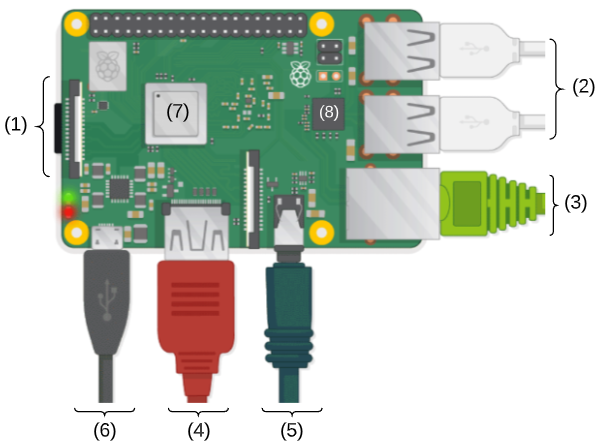
\includegraphics[scale=0.75]{img/raspberry4.png}
 \end{center}
 \caption{Diagrama de componentes de la Raspberry Pi 3. Tomada de \cite{defraspberry} \label{raspberrypng}}
\end{figure}

La Figura anterior permite observar el diagrama de los componentes de una Raspberry Pi y son listados así:
\begin{multicols}{2}
\begin{itemize}
    \item [(1)] Ranura para tarjeta micro SD
    \item [(2)] Puertos de conexión USB
    \item [(3)] Puerto de conexión Ethernet
    \item [(4)] Puerto de conexión HDMI
    \item [(5)] Puerto de conexión de audio (Jack)
    \item [(6)] Puerto de conexión de alimentación
    \item [(7)] Microprocesador
    \item [(8)] Memoria RAM
\end{itemize}
\end{multicols}

\subsection{Sistemas embebidos} \label{subsectionembebidos}

También conocidos como sistemas empotrados, son sistemas de computación diseñados para propósitos especializados de reacción con el entorno, es decir que en tiempo real puedan desempeñar unas pocas funciones dedicadas y al contrario que los computadores, no están diseñados para ser  programados por los usuarios finales. Esto quiere decir que el usuario final no modificará o reemplazará la funcionalidad del sistema al agregar o quitar software. Mas sin embargo, podrá tomar decisiones concernientes a la ejecución de los procesos que éste realice \cite{embebido}. Por lo general, en un sistema embebido, los componentes suelen estar unidos mediante una única placa base que se puede programar mediante lenguajes de programación como ``C'', ``C++'', ``Python'', e incluso ``java''.

\subsubsection{Componentes}

En el listado de componentes centrales de un sistema de este tipo suele encontrarse:

\begin{itemize}
    \item \textbf{Microprocesador:} En términos generales es un circuito integrado perteneciente a la CPU considerado como el ``Cerebro'' en un sistema informático (ver figura \ref{atmegapng}). Este es el encargado de ejecutar el sistema operativo, programas y las aplicaciones de usuario.
    
\begin{figure}[H]
 \begin{center}
 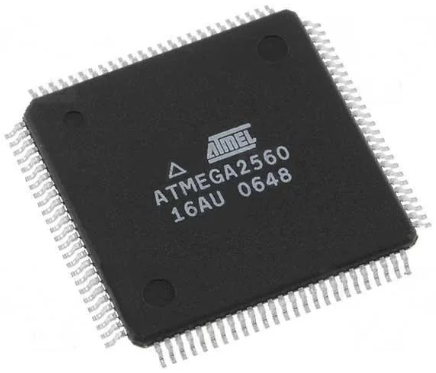
\includegraphics[scale=0.65]{img/atmega.png}
 \end{center}
 \caption{Ejemplar de microprocesador ATMega2560. Tomado de \cite{arduinodef}.
 \label{atmegapng}}
\end{figure}

    \item \textbf{Memoria principal:} Para este tipo de dispositivos comúnmente se emplea una memoria RAM. Es la memoria interna del sistema de cómputo en donde se almacenan las instrucciones y los datos que serán procesados por la CPU con quien se comunica mediante el bus de datos y el bus de direcciones.
    
    \item \textbf{Microcontrolador ($\mu C$):} Es un circuito integrado programable, con la capacidad de ejecutar las ordenes almacenadas en la memoria interna. Típicamente, la arquitectura general de un microcontrolador comercial poseerá dispositivos de entrada y salida como los conversores ADC, temporizadores y buses de interfaz como el $I_2C$ y $CAN$ (ver figura \ref{mucpng}). Los microcontroladores suelen incluir un lenguaje de programación integrado con instrucciones de procesadores especializados como lo es en el caso de Arduino y BASIC.
    
\begin{figure}[H]
 \begin{center}
 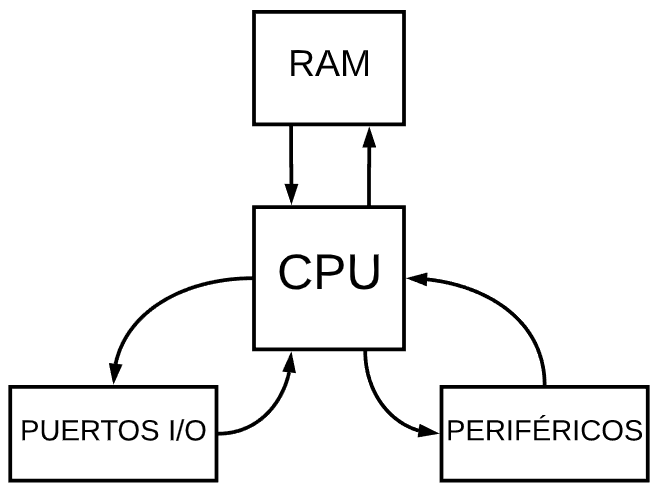
\includegraphics[scale=0.65]{img/muc.png}
 \end{center}
 \caption{Diagrama de comunicación con periféricos. \label{mucpng}}
\end{figure}

    
    A diferencia de un microprocesador, estos pueden ser convertidos en una computadora funcional mediante la conexión de circuitos integrados externos de apoyo y conexión a los sistemas de información y alimentación que requiera. Por su parte, el microprocesador requerirá que otros chips o módulos se encarguen de estas tareas.\\
    
    \item \textbf{Unidad de procesamiento digital de señales (DSP):} Por medio de esta se logra la manipulación matemática y digital de una señal en pro de modificarla, analizarla o mejorarla en algún sentido. Las señales entrantes y salientes pasan por un proceso de conversión analógica $\Longleftrightarrow$ digital mediante los conversores ADC y DAC. Estas unidades se obtienen al interconectar hardware, software e instrucciones optimizadas para aplicaciones numéricas. Gracias a esto, es especialmente útil para aplicaciones de procesamiento y representación de señales analógicas en tiempo real.
\end{itemize}

En resumen, estos componentes reflejan la Unidad de Central de Procesamiento (CPU). En lo que respecta a la visualización de datos se tienen dispositivos de salida como las pantallas LCD, gráficas, o interfaces alfanuméricas.\\

Por último, además de su estructura física, la parte tangible de los sistemas embebidos comprende a los actuadores, que es todo tipo de elemento electrónico que pueda ser manipulado por señales de control; entre los más comunes son los motores de corriente continua mediante pulsos modulados (PWM).

\subsubsection{Sistema de tiempo real}

Son sistemas informáticos de interacción con el entorno físico que reaccionan a estímulos del entorno en  determinados instantes de tiempo ($Inputs$). Según la aplicación se puede tratar de tiempo real crítico (o duro) y acrítico (o suave); respectivamente quiere decir que los tiempos de respuesta pueden determinar si la reacción al estímulo debe realizarse explícitamente en  un intervalo de tiempo específico o no.

Entre los dispositivos más usados para los sistemas de tiempo real crítico y acrítico se puede mencionar a Arduino; en particular, para este último caso y, en algunas ocasiones, para el primer caso.

Debido a su acogida en el mercado, simplicidad de uso y codificación, y su uso en aplicaciones de prototipado y aprendizaje en tareas especializadas, es un gran postor como microcontrolador  en sistemas embebidos. Mediante la conexión de diferentes sensores, módulos y componentes de hardware se pueden lograr tareas funcionales de fácil aplicación y manipulación. Un esquema de ejemplo para un sistema de tiempo real crítico se puede ver en la Figura \ref{esquematico1png}.

\begin{figure}[H]
 \begin{center}
 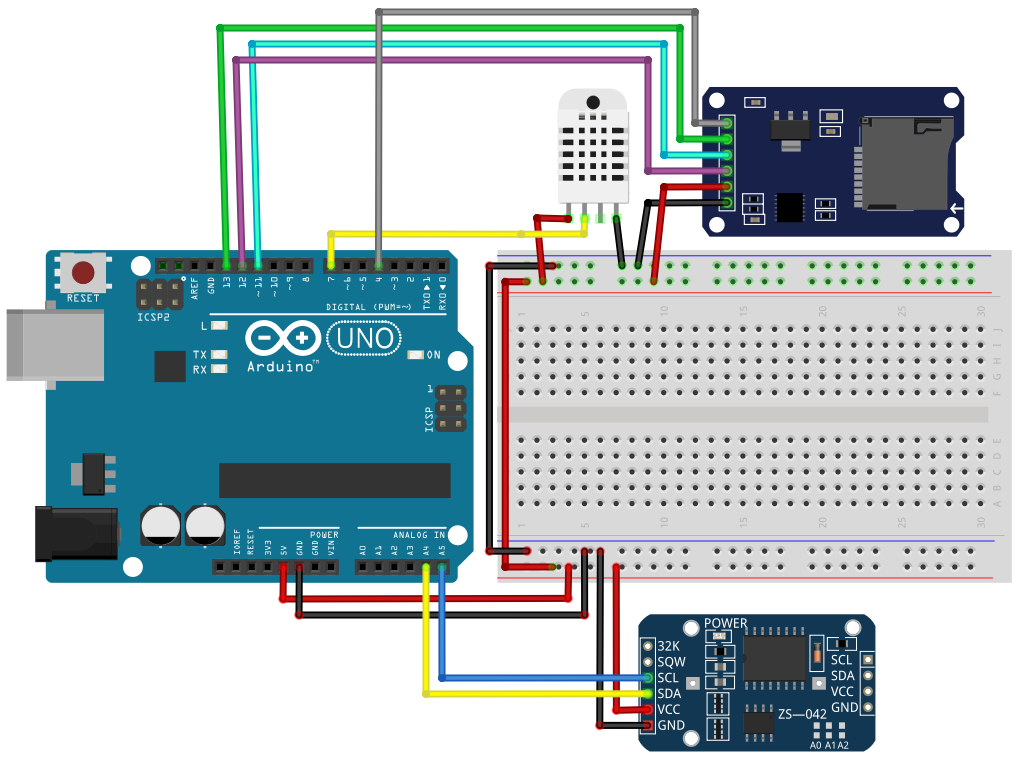
\includegraphics[scale=0.35]{img/esquematico1.png}
 \end{center}
 \caption{Ejemplo de esquemático de conexión de Arduino para medición y registro de temperatura y hora. \label{esquematico1png}}
\end{figure}

% Un ejemplo que ilustra los puntos anteriores es el de un robot que necesita tomar una pieza de una banda sinfín. Si el robot llega tarde, la pieza ya no estará donde debía recogerla, por tanto, el trabajo se llevó a cabo incorrectamente, aunque el robot haya llegado al lugar adecuado. Si el robot llega antes de que la pieza llegue, la pieza aún no estará ahí y el robot puede bloquear su paso.

\subsubsection{Aplicaciones}

Para el desarrollo de aplicaciones con sistemas embebidos y prototipos existen plataformas desarrolladas como Raspberry Pi, Arduino, mbed, BeagleBone, entre otros.\\

Los programas de sistemas embebidos se enfrentan usualmente a tareas de procesamiento en tiempo real por lo que para ejemplificar aplicaciones de estos sistemas electrónicos se mencionan las siguientes:

\begin{itemize}
    \item  \textbf{Sistemas automatizados de alimentación para vacas de alta producción de leche}
    En este trabajo de grado, se utiliza un sistema electrónico que se encarga de registrar si un animal ha ingerido su porción fija de alimento en su totalidad, y se encarga de registrar  el restante en caso que se presente esa situación. Para mayor información ver \cite{aguero}.  
    \item  \textbf{Dispensador automático de comida para mascotas, programable y controlado remotamente}
    En este trabajo de grado de la Universidad del Valle se utiliza un microcontrolador $ATMEGA644$ para procesar las indicaciones  y activar los mecanismos de dosificación de alimento en porciones y horas determinadas. Tomado de \cite{univalle}.\\
    \item  \textbf{Maquinaria de pesado industrial y doméstica} 
    Entre las aplicaciones más comunes de un sistema embebido sencillo se encuentran las básculas de pesaje tanto doméstico como industrial.
    \item  \textbf{Impresoras 3D}
    En la actualidad es posible fabricar impresoras 3D sencillas mediante el uso de sistemas embebidos con micro controladores como Arduino y módulos adicionales de control para el manejo de los motores que maniobran en el espacio de impresión.
    \item  \textbf{Robótica}
    El uso de estos sistemas es altamente usado en la industria para tareas sistematizadas como el control y la automatización de procesos en sistemas de control de lazo cerrado y sobre todo en sistemas de tiempo real crítico como en las cintas transportadoras.
\end{itemize}

% \textbf{BITÁCORA DEL TIEMPO 12 SEPTIEMBRE 2019 8:30PM 
% Hacer la comparacion entre ardino y la resperry pi cuando mencione la parte de escoger al microprocesador pero eso sería mas adelante en el capitulo 5 o 6}

% \subsubsection{Microprocesadores}


% \section{Adquisición de datos} % 
% 
% 

Como se mencionó en la Sección \ref{subsectionembebidos}, los sistemas electrónicos están en la capacidad de reaccionar a los estímulos del entorno. Esto hace referencia a los datos y señales de entrada provenientes de elementos electrónicos que suministran tal información. Para medir los datos que luego serán procesados e interpretados en acciones de la unidad central de procesos de un sistema computacional es necesario hacer uso de estos elementos:

\subsection{Sensores}

Son dispositivos que pueden variar sus propiedades ante magnitudes físicas o químicas del medio. Esto significa que pueden detectar su presencia y también su medida. A las variables medidas se les denomina variables de instrumentación y al transformarlas mediante el uso de un transductor se convierten en variables eléctricas. Un transductor es un elemento que recibe variaciones de energía y están en la capacidad de representarlas mediante otras variaciones de energía de salida \cite{instrum}. A diferencia de los transductores, los sensores están en contacto constante con la variable de instrumentación a la que se encuentran expuestos. Con base en esto se puede establecer que los sensores ``traducen''  o adaptan una señal de entrada para que otros dispositivos puedan interpretarla.\\

%%% Tek

Las señales de entrada son definidas como una manifestación abstracta, física o simbólica de información como por ejemplo las señales de audio, imágenes, manifestaciones climatológicas y del medio, físicas y químicas. Como los sensores entregan una variación de energía en la salida que a su vez representa la conversión de una señal de entrada de una variable de instrumentación en particular, esta debe ser modificada para que pueda ser interpretada correctamente por otros dispositivos de análisis de datos. Para ello es posible que sea necesario hacer uso de un acondicionamiento de la señal para representar la variable mediante una diferencia de potencial y dependiendo del tipo de sensor, es probable que se deba incluir una etapa de conversión de señal analógica o digital. \cite{instrum}.

\subsubsection{Clasificación}

Para determinar si un sensor requiere de una etapa de conversión ADC, los sensores son clasificados por sus características, que pueden ser del tipo de señal analógica o digital.

\begin{itemize}
    \item \textbf{Sensores de señales analógicas}
    Los sensores analógicos miden señales que están definidas para todos los valores de tiempo en un intervalo continuo. Esto quiere decir que para todo instante de tiempo existirá una señal de salida proporcional a un valor de magnitud de la variable medida \cite{benitez}.
    
    \item \textbf{Sensores de señales digitales}
    Los sensores digitales miden señales que están definidas por valores discretos, es decir que representan una señal mediante una variación discontinua en el tiempo y solo pueden tener un número finito de valores discretos \cite{benitez}.
\end{itemize}


\subsubsection{Características técnicas}
\begin{itemize}
    \item \textbf{Linealidad}
    Se dice que un sensor es lineal si su curva de calibración se asemeja a una línea recta. Esto quiere decir que su comportamiento de medida es lineal entre su variable de medida y la señal de salida que entrega el sensor.
    
    \item \textbf{Precisión}
    Es la capacidad de un instrumento de medición de entregar valores aproximadamente iguales a medida que se repiten los eventos de medición bajo las mismas condiciones.
    
    \item \textbf{Error}
    Es la discrepancia existente entre el valor medido (valor real) y el valor teórico de medición (valor ideal o de referencia).
    
    \item \textbf{Exactitud}
    Es la capacidad de un instrumento de medición de entregar valores que se aproximen al valor verdadero de la magnitud de medida.
    
\end{itemize}

% \subsubsection{Clasificación}
% ==================================================================
% ==================================================================
% ==================================================================
%  **********YO CREO QUE ESTA PARTE DE SOFTWARE VA MEJOR EN EL TRATAMIENTO DE LOS DATOS************************************.
% \subsection{Software}

% Se entiende como Software a todo soporte lógico e intangible necesario que hacen posible la realización de tareas especificas. Según el estándar 729 de la IEEE, se entiende como  el conjunto de programas, procedimientos, reglas, documentación y datos asociados que forman parte de las operaciones de un sistema de computo. Entre los componentes lógicos se puede hacer mención de de aplicaciones informáticas, el sistema operativo que permite que los programas funcionen correctamente y los programas de interfaz de usuario. \\

% Por lo general, el software se escribe en lenguajes de programación de alto nivel, es decir que son herramientas de programación fáciles y eficientes para los programadores debido a su semejanza al lenguaje natural, por su parte los sistemas de computo ejecutan estos programas en lenguaje maquina. La traducción entre estos lenguajes se realiza mediante un compilador que se encarga de ``traducir'' las instrucciones.

% \subsubsection{Clasificación}
% \begin{itemize}

%     \item \textbf{Sistema: }
%     El es tipo de software de alto nivel que separa las acciones del usuario en comparación de las acciones de bajo nivel que debe ejecutar el sistema de computo con respecto a su memoria, procesador, etc.
    
%     \item \textbf{Programación: }
%   Son las herramientas que le facilitan al programador programar los algoritmos informáticos mediante lenguajes de programación de manera aplicada. A groso modo poseen Editores de texto, compiladores, interpretes y entornos de desarrollo que cuentan con interfaces gráficas para el usuario.
    
% \end{itemize}

% % \subsubsection{Características}
% % \begin{itemize}
% %     \item \textbf{Programación o Codificación}
% % % \end{itemize}
% % 



% \subsubsection{Codificación}
% El proceso para  diseñar software se logra con el objetivo de idear la forma en que las acciones se realizarán en el marco de un proyecto para solventar una necesidad en particular. Hoy en día se considera programación al proceso de escritura de algoritmos computacionales mediante un editor de texto o herramienta integrada como los lenguajes de programación entre los que se encuentran Python, C y C++.\\

% Los algoritmos son un conjunto de instrucciones o reglas predefinidas de manera ordenada que permiten llevar a cabo una actividad mediante pasos consecutivos secuenciales o paralelos de manera no ambigua para poder realizar una actividad \cite{algoritmo}. Los algoritmos computacionales son algoritmos más sofisticados y precisos que permiten aprovechar las nuevas tecnologías y que al depender de una memoria limitada deben ser lo mas optimizados posible para que puedan procesar grandes cantidades de datos con capacidades finitas y generalmente a bajo costo. 

% ****************************************************


% \section{Hardware} 

El hardware se entiende como todo componente físico y tangible de un sistema de cómputo. En un proyecto  electrónico, el hardware abarca desde los circuitos eléctricos, la armadura del circuito y el conjunto de elementos, sensores, y actuadores que permiten ejecutar el software y las acciones lógicas necesarias para dar solución a una necesidad en particular.\\

\textit{\textbf{Observación: }En la escala de este proyecto, el hardware comprende en su mayoría la estructura física del prototipo, los sensores y los actuadores  manipulados por señales de control.}

\subsection{Actuadores}
\subsubsection{Actuadores Electrónicos}
\begin{itemize}
    \item \textbf{Servo}
    Los servomotores son motores similares a los de corriente directa con la posibilidad de ubicarse en una posición especifica dentro de su rango de operación. Están conformados por un motor, un mecanismo reductor y un circuito de control. Generalmente poseen potencia proporcional para cargas mecánicas; por lo tanto no consumen mucha energía a diferencia de otros ejemplares como los motores paso a paso.
\end{itemize}
\subsubsection{Actuadores Mecánicos}
\begin{itemize}
    \item \textbf{Mecanismo Biela-Manivela}
    Este mecanismo permite transformar movimiento circular en movimiento de traslación o viceversa. De manera esquemática, el mecanismo se crea con dos barras unidas por un par cinemático. Uno de los extremos de la barra que rota (la manivela) esta unida a un punto fijo siendo éste el centro de giro; su otro extremo está unido a la biela. El extremo restante de la biela se encuentra unido a un pistón que se mueve en línea recta.
    \item \textbf{Mecanismo de Tornillo sin Fin}
    Este mecanismo es descrito previamente en la sección \ref{endscrew}.
    
\end{itemize}

% \section{Tratamiento de datos}
% \subsection{Software}
% \subsubsection{Codificación}

\section{Tratamiento de datos} % 
% 
% 

\subsection{Software}

Se entiende como Software a todo soporte lógico e intangible necesario que hacen posible la realización de tareas especificas. Según el estándar 729 de la IEEE, se entiende como  el conjunto de programas, procedimientos, reglas, documentación y datos asociados que forman parte de las operaciones de un sistema de cómputo. Entre los componentes lógicos se puede hacer mención de aplicaciones informáticas, el sistema operativo que permite que los programas funcionen correctamente y los programas de interfaz de usuario. \\

Por lo general, el software se escribe en lenguajes de programación de alto nivel, es decir que son herramientas de programación fáciles y eficientes para los programadores debido a su semejanza al lenguaje natural. Por su parte los sistemas de cómputo ejecutan estos programas en lenguaje máquina. La traducción entre estos lenguajes se realiza mediante un compilador que se encarga de ``traducir'' las instrucciones.

\subsubsection{Clasificación}
\begin{itemize}

    \item \textbf{Sistema: }
    Es el tipo de software de alto nivel que separa las acciones del usuario en comparación de las acciones de bajo nivel que debe ejecutar el sistema de cómputo con respecto a su memoria, procesador, etc.
    
    \item \textbf{Programación: }
   Son las herramientas que le facilitan al programador programar los algoritmos informáticos mediante lenguajes de programación de manera aplicada. A grosso modo poseen Editores de texto, compiladores, intérpretes y entornos de desarrollo que cuentan con interfaces gráficas para el usuario.
    
\end{itemize}

\subsubsection{Codificación de algoritmos en OSS}

El Software de Código Abierto OSS (Open Source Software) es un concepto relativamente reciente que abarca un modelo de desarrollo de software basado en colaboración abierta en Internet, donde un propietario de software permite a los usuarios utilizar, cambiar y redistribuir el software para cualquier propósito. \cite{Defopensource}.

El proceso para  diseñar software se logra con el objetivo de idear la forma en que las acciones se realizarán en el marco de un proyecto para solventar una necesidad en particular. Hoy en día se considera programación al proceso de escritura de algoritmos computacionales mediante un editor de texto o herramienta integrada como los lenguajes de programación entre los que se encuentran Python, C y C++.

Los algoritmos son un conjunto de instrucciones o reglas predefinidas de manera ordenada que permiten llevar a cabo una actividad mediante pasos consecutivos secuenciales o paralelos de manera no ambigua para poder realizar una actividad \cite{algoritmo}. Los algoritmos computacionales son algoritmos más sofisticados y precisos que permiten aprovechar las nuevas tecnologías y que al depender de una memoria limitada deben ser lo mas optimizados posible para que puedan procesar grandes cantidades de datos con capacidades finitas y generalmente a bajo costo.

% =========================================================
    
% =========================================================


\subsection{Data Clustering}

\subsubsection{Bases de datos digitales}
Es un conjunto de datos interrelacionados y almacenados de forma ordenada y sistemática (Ver Figura \ref{databasepng}) para un uso posterior\cite{database}. Debido al desarrollo tecnológico de la informática y la electrónica, estas bases de datos suelen ser digitales y por lo general se almacenan en la nube (Cloud). Por otra parte, es considerado un modelo de almacenamiento de datos basado en redes de computadoras, donde los datos están alojados en espacios de almacenamiento virtualizados \cite{cloud}.

	\begin{figure}[H]
		\begin{center}
			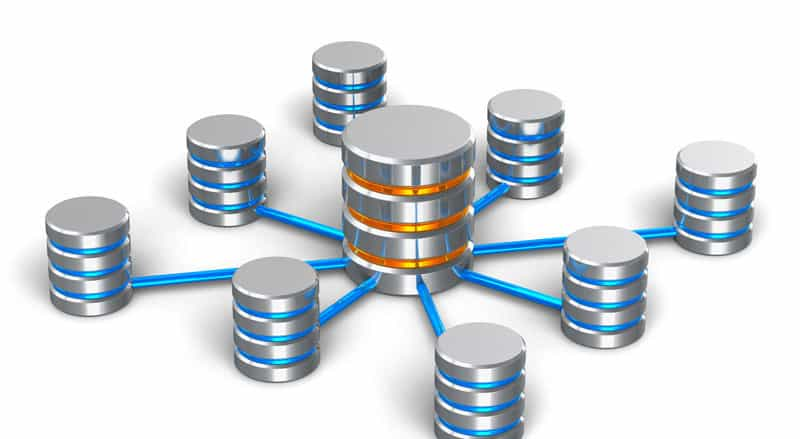
\includegraphics[scale=0.5]{img/databasepng.png}
		\end{center}
	\caption{Base de datos. Tomada de \cite{googlepics}. \label{databasepng}}
	\end{figure}

% \subsubsection{Cloud}

% %%% Tek

% La nube, también denominada como ``Cloud Storage" (Ver Figura \ref{cloudpng}), se refiere tanto a las aplicaciones entregadas como servicios a través de Internet y el software del hardware y sistemas en los centros de datos que proporcionan estos servicios \cite{cloud2}.
% 	\begin{figure}[H]
% 	\begin{center}
% 		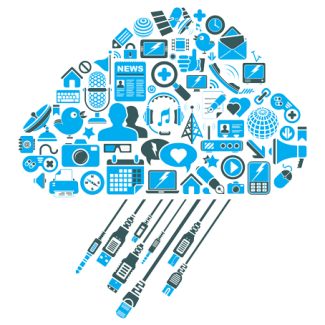
\includegraphics[scale=0.45]{img/cloud.png}
% 	\end{center}
% 	\caption{Almacenamiento en nube. Tomada de \cite{googlepics}. \label{cloudpng}}
% 	\end{figure}


% \section{Nuevas tecnologías} % 
% 
% 
\begin{itemize}

\item \textbf{Arduino}

Es una plataforma electrónica de código abierto basado en software y hardware de fácil uso. Las placas de Arduino están en la capacidad de leer entradas, manipular sensores y transmitir información de manera remota, entre otros. Estas placas son reprogramables mediante una serie de instrucciones al microcontrolador y se pueden programar con múltiples lenguajes de programación \cite{arduinodef}.

\item \textbf{PLC}

Es una computadora lógica y programable utilizada para automatizar procesos electromecánicos, electro-neumáticos y electro-hidráulicos especialmente en líneas de montaje o procesos de producción\cite{plcref} .

\item \textbf{Raspberry Pi}

Son microordenadores de placa reducida de bajo costo que tiene como objetivo estimular la enseñanza de la informática aunque tiene usos incluso profesionales como en la robótica. A este dispositivo se le pueden agregar periféricos al igual que a un ordenador de escritorio y puede ser usado  como tal. Sus usos abarcan desde sistemas de cómputo básico, análisis de datos, representación de imágenes y vídeo, y aplicaciones básicas de automatización \cite{piref}.

%CARACTERÍSTICAS Y PROPIEDADES DE CADA UNO

%TABLA COMPARATIVA

\end{itemize}


% % animales

% % . Desde el uso de 

% % Es necesario recalcar que todas las aplicaciones y herramientas de trabajo que relacionan la Ingeniería Electrónica y las ciencias agropecuarias

% \section{Conceptos adicionales} \input{docs/conceptad.tex} \label{concepadic}
 
% %  \textit{\textbf{Bitácora del tiempo: 13/09/19  Falta acabar esta sección del capitulo 4. Yo creo que tendría que adicionar otra sección o esta misma en donde explico los conceptos teóricos del infrarojo, del rfid, del pwm, de la celda de carga para no tener que explicarlos a modo de teoría en el capitulo 5}}
 
% \begin{itemize}

% 	\item \textbf{HMI:} Por sus siglas en inglés, ``Human-Machine Interface'', se refiere a la interfaz de interacción entre máquinas y humanos (Ver Figura \ref{hmipng}), aplicable a los sistemas de automatización de procesos \cite{hmi}.
	
% 	\begin{figure}[H]
% 	\begin{center}
% 		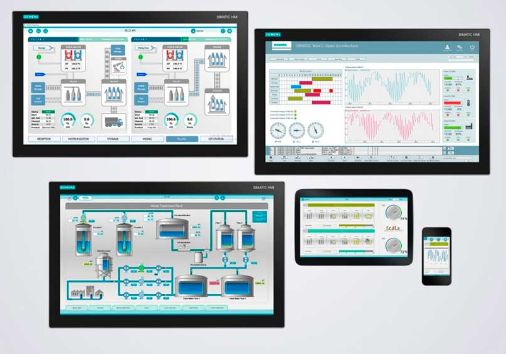
\includegraphics[scale=0.65]{img/hmi.png}
% 	\end{center}
% 	\caption{Ejemplos de Human-Machine Interface. Tomada de \cite{googlepics}. \label{hmipng}}
% 	\end{figure}
	
% %%% Tek	
	
% 	\item \textbf{RFID:}
% 	 La identificación por radiofrecuencia (Ver Figura \ref{rfid1png}), es un sistema reprogramable de almacenamiento, lectura y recuperación de datos de manera inalámbrica mediante etiquetas, tarjetas o transpondedores en general, que pueden ser adheridas a productos, animales e incluso a personas sin necesidad de alimentación interna. Este sistema tiene una gran variedad de aplicaciones entre las cuales se pueden mencionar logísticas de distribución, servicios industriales, control de acceso, entre otros \cite{rfid1}. \\
% % 	 Estas aplicaciones tienen en común la posibilidad de relacionar atributos, caracteristicas o datos especificos con respecto a un objeto en especifico.\\
 
% 	\begin{figure}[H]
% 	\begin{center}
% 		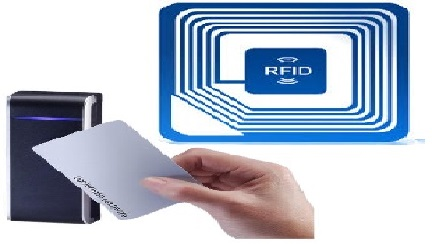
\includegraphics[scale=0.8]{img/rfid1.png}
% 	\end{center}
% 	\caption{Sistemas RFID. Tomada de \cite{googlepics}. \label{rfid1png}}
% 	\end{figure}
	
% 	\item \textbf{Modulación por Ancho de Pulsos (PWM)}
	
% 	El uso del PWM en motores eléctricos es una técnica utilizada para regular la velocidad de giro. Mantiene el par motor constante y no supone un desaprovechamiento de la energía eléctrica. Es usado tanto en corriente directa como alterna e implica que un momento en alto (High) el motor está siendo alimentado y un momento en bajo (Low) el motor está apagado o desconectado.
% % 	\begin{figure}[H]
% % 	\begin{center}
% % 		\includegraphics[scale=0.99]{img/pwm.png}
% % 	\end{center}
% % 	\caption{Sistemas RFID. \label{rfid1png}}
% % 	\end{figure}
	
% 	\item \textbf{Puente de Wheatstone}
	
% 	Es un circuito eléctrico que se utiliza para medir resistencias desconocidas mediante el equilibrio de los brazos del puente. Estos están constituidos por cuatro resistencias que forman un circuito cerrado, siendo una de ellas la resistencia bajo medida. En este proyecto, esta resistencia bajo medida representa a la celda de carga que permite determinar el valor de las masas en cuestión (la cantidad de alimento y el peso del animal).

% \end{itemize}
